\section{Progettazione dell'array di patch}
Una volta soddisfatte le specifiche per il singolo patch rettangolare, è necessario cercare di soddisfare anche le restanti, relative all'array. \\ 
Per fare questo è possibile agire su due fattori relativi all'array: il numero degli elementi che formano l'array e la spaziatura tra gli elementi. Per calcolare il numero di elementi che formano l'array ci si deve riferire alla specifica del guadagno massimo dell'array, la relazione che lo lega con il guadagno del singolo patch permette di ottenere il numero di elementi che formano l'array considerando un'illuminazione uniforme.
\begin{align*}
G^{(array)}_{max} = (K+1) G^{(patch)}_{max}
\end{align*}
\begin{align}
\label{eq:m}
\Rightarrow M = K + 1 =  \biggr\lceil \frac{G^{(array)}_{max}}{G^{(patch)}_{max}} \biggr\rceil = \lceil 7.71 \rceil = 8
\end{align}
dove:
\begin{itemize}
\item $G^{(array)}_{max}$ è dato dalla specifica di progetto: $16 dB$
\item $G^{(patch)}_{max}$ è quello ottenuto nella figura \ref{img:polar}: $7.26 dB$
\end{itemize}
Il numero di elementi trovato nell'equazione \ref{eq:m} rappresenta il numero \emph{minimo} di elementi che possono formare l'array a illuminazione uniforme; in questo lavoro, però, si studia la progettazione di un array a illuminazione simmetrica, pertanto la scelta del numero \emph{minimo} di elementi si opera attraverso le seguenti equazioni:
\begin{align}
\label{eq:mopt}
N = \biggr\lceil \frac{M-1}{2} \biggr\rceil = 4 \Rightarrow M = 2N + 1 = 9
\end{align}

Il numero di elementi \emph{minimo} trovato nella (\ref{eq:mopt}) soddisfa il requisito sul guadagno massimo dell'array, quest'ultimo passaggio è stato necessario al fine di poter applicare la sintesi di \cheby. In questo modo sarà possibile calcolare il numero ottimo di elementi che formano l'array e la loro distanza. \\
Restano quindi da soddisfare gli ultimi due requisiti che riguardano \emph{il rapporto tra l'ampiezza massima del lobo principale e quella del lobo secondario} e \emph{l'angolo a metà potenza (BW)}. \\

\subsection{Sintesi di \cheby}
La sintesi di \cheby è stata automatizzata attraverso un programma in Python, di cui è allegato il codice. \\[1cm]

Il primo script contiene le funzioni che calcolano i parametri di \cheby, i coefficienti di alimentazione e il fattore d'array e eseguono la sintesi dando in output tutti i risultati.
\begin{minted}[linenos=true,frame=leftline,xleftmargin=0.5cm,fontsize=\footnotesize]{python}
import math
from pylab import*

# the function takes in input the number of array elements "n" and 
# the attenuation of the secondary lobes compared to the main lobe
def chebyParam( n , r ):
    n = float(n)
    r = float(r)
    iterator = math.cosh(1/n * math.acosh(r))
    a = (( iterator - 1 ) / 2 ).real
    b = (( iterator + 1 ) / 2 ).real
    #returns the list of chebyshev's parameters
    return [ a , b ]

#chebyshev's parameters and optimized distance value btw array elements
def chebyParamOptimized(n , r , k0 ):
    n = float(n)
    r = float(r)
    iterator = math.cosh(1/n * math.acosh(r))
    a = (( iterator - 1 ) / 2 ).real
    b = (( iterator + 1 ) / 2 ).real
    optimized_dist = ( 2*math.pi - math.acos((1 - a)/b)) / k0
    output = open("valori_a_b.txt",'a')
    output.write(" a = " + str(a) + " b = " + str(b) + "  N = " + str( n*2+1) + "\n")
    output.close()
    return [ a , b , optimized_dist]

# the function takes in input the chebyshev's parameters and returns the 
# excitation coefficients

def excitCoeff( n , a, b):
    if n not in range(2,5):
        raise Exception("The number isn't in the range [ 2 , 4 ]")
    # 5 elements array
    def five_elem():
        k0 = 2*a**2 + b**2 - 1
        k1 = 4*a*b/2
        k2 = b**2/2
        return [ k0 , k1 , k2 ]
    #7 elements array
    def seven_elem():
        k0 = 4*a**3 + 6*a*b**2 - 3*a
        k1 = ( 12*a**2*b +3*b**3 - 3*b )/2
        k2 = ( 6*a*b**2 )/2
        k3 = b**3/2
        return [ k0 , k1 , k2 , k3 ]
    #9 elements array
    def nine_elem():
        k0 = -8*a**2 + 8*a**4 - 4*b**2 + 3*b**4 + 24*a**2*b**2 +1
        k1 = (24*a*b**3 + 32*a**3*b - 16*a*b)/2
        k2 = (4*b**4 - 4*b**2 + 24*a**2*b**2)/2
        k3 = 8*a*b**3/2
        k4 = b**4/2
        return [ k0 , k1 , k2 , k3 , k4 ]

    feed_coeff = { 2 : five_elem , 3 : seven_elem , 4 : nine_elem }
    return feed_coeff[n]()

#the function takes in input the excitation coefficients, the distance between array elements, 
#the angle of orientation
#returns the array factor

def arrayFactor( coeff , dist , angle , k0 ):
    u = k0 * dist * cos((angle*pi)/180)
    f = zeros(len(angle))
    for item in range(0,len(angle)):
        f[item] = coeff[0]
        for item2 in range(1,len(coeff)):
            f[item] = f[item] + 2*coeff[item2]*cos(item2*u[item])
    return f


# Chebyshev sysnthesis

def chebyshevSynthesis( f0 , r , angle , gain , n ):

    gain = 10**(array(gain)/10)
    c = float(3*(10**8))
    #wave length
    r = 10**(r/20)
    lambda_0 = c/float(f0)
    k0 = 2*math.pi/lambda_0
    psi = 90 - np.array(angle)
    m = int(ceil(( n-1 )/2))
    params = chebyParamOptimized( m , r , k0)
    excitation_coeff = excitCoeff( m, params[0] , params[1] )
    array_factor = np.array(arrayFactor( excitation_coeff, params[2] , psi , k0))
    #square absolute value of the array factor
    abs_array_factor = abs(np.array(array_factor))**2

    # the sum of the absolute values of the excitation parameters
    sum_coeff = sum( abs(array(excitation_coeff))**2)*2 - abs(excitation_coeff[1])**2 
    
    array_factor_gain = abs_array_factor/float(sum_coeff)
    #the gain of the antenna
    system_gain = array_factor_gain * gain
    db_system_gain = 10*log10(system_gain)

    
    max_gain = max(db_system_gain)
    
    db_3_gain = 0
    teta_3_db = -1

    for  item in range(1, len(angle)):
        if db_system_gain[item] == db_3_gain :
            teta_3_db = angle[item]
            break
        elif db_system_gain[item] < db_3_gain:
            teta_3_db = angle[item - 1]
            break
    

    if teta_3_db == -1 :
        print(" Impossible to calculate the beamwidth ")
    print(teta_3_db)
    bw = 2*teta_3_db

    return [ array_factor , array_factor_gain , system_gain , max_gain , bw ]


def chebySynthesisDistance( f0 , r , angle , gain , n , dist ):
    c = float(3*10**8)
    r = 10**(r/20)
    lambda_0 = c/float(f0)
    k0 = 2*math.pi/lambda_0
    psi = 90 - array(angle)
    m = int(ceil((n-1)/2))
    params = chebyParam( m , r )
    excitation_coeff = excitCoeff( m , params[0] , params[1] )
    array_factor = arrayFactor(excitation_coeff , dist , psi , k0 )
    abs_array_factor = abs(array_factor)**2
    sum_coeff = sum(abs(array(excitation_coeff))**2)*2 - abs(excitation_coeff[1])**2
    array_factor_gain = abs_array_factor/float(sum_coeff)
    system_gain = array_factor_gain*gain
    db_system_gain = 10*log10(system_gain)
    max_gain = max(system_gain)
    db_max_gain = max(db_system_gain)
    db_3_gain = db_max_gain - 3
    print(db_system_gain)
    teta_3_db = -1
    for  item in range(0, len(angle)):
        if db_system_gain[item] == db_3_gain: 
            teta_3_db = angle[item]
            break
        elif db_system_gain[item] < db_3_gain:
            teta_3_db = angle[item - 1]                                                         
            break
        
    if teta_3_db == -1 :
        print(" Impossible to calculate the beamwidth ")

    bw = 2*teta_3_db
    return [ array_factor , array_factor_gain , system_gain , max_gain , bw ]

def plot_function(axes,values , names ):
    m = values[0]
    g=[]
    for item in axes:
        g.append(-1*item)
    g = g[::-1]
    axes = g + axes
    values = array(list(values[::-1])+list(values))
    plot(axes,values)
    ylim(-60,35)
    xlim(-90,90)
    annotate(str(m)[0:5], xy=(5, m+6), xytext=(5, m+6),bbox=dict(boxstyle="larrow", fc="w"), rotation = 35)
    grid(True)

    ylabel(names[0])
    xlabel(names[1])
    title(names[2])
\end{minted}

Il seguente script genera i grafici del fattore d'array e del guadagno totale dell'antenna.
\begin{minted}[linenos=true,frame=leftline,xleftmargin=0.5cm,fontsize=\footnotesize]{python}
import antenna_package
import math
from pylab import*

r = float(20)
f0 = 5.8*10**9
file_gain = open("gainTotal.txt",'r')
file_angles = open("gain_angoli.txt",'r')

gain = []
angles = []
while True:
    line = file_gain.readline()
    if not line:
        break
    gain.append(float(line))
file_gain.close()

while True:
    line = file_angles.readline()
    if not line:
        break
    angles.append(float(line))
file_angles.close()

for item in gain:
    item = 10**item/10

n = [ 5,7,9 ]
array_factors = zeros((len(n),len(gain)))
array_factors_gain = zeros((len(n),len(gain)))
system_gain = zeros((len(n),len(gain)))
max_gain = zeros(len(n))
beam_width = zeros(len(n))
output = open("beamwidth.txt",'wa')
for item in range(0,len(n)):
    synthesis_result = antenna_package.chebyshevSynthesis( f0, r , angles , gain, n[item] )
    array_factors[item] = synthesis_result[0]
    array_factors_gain[item] = synthesis_result[1]
    system_gain[item] = synthesis_result[2]
    max_gain[item] = synthesis_result[3]
    beam_width[item] = synthesis_result[4]

for item in range(0,len(n)):
    output.write("N = " + str(n[item]) + " bw = " + str(beam_width[item]) + "\n")
output.close()
max_gain_db = 10*log10(max_gain)
array_factors_abs = abs(array_factors)
array_factors_abs_db = 20*log10(array_factors_abs)
array_factors_gain_db = 10*log10(array_factors_gain)
system_gain_db = 10*log10(system_gain)

g = []
for item in angles:
    g.append(-1*item)
g=g[::-1]
axes = g + angles
a = list(array_factors_abs_db[2][::-1]) + list(array_factors_abs_db[2])

for item in range(0,len(n)):
    names_array_factors = [ "db","angle","Array factor absolute value for " + str(n[item]) + " elements"]    
    figure()
    antenna_package.plot_function(angles,array_factors_abs_db[item],names_array_factors)
    show()
    names_system_gain = ["db","angle"," Gain of the " + str(n[item]) + " elements array patch antenna"]
    figure()
    antenna_package.plot_function(angles,system_gain_db[item],names_system_gain)
    show()
\end{minted}

L'ultimo script genera i grafico dell'andamento del beamwidth in funzione della spaziatura tra i patch.
\begin{minted}[linenos=true,frame=leftline,xleftmargin=0.5cm,fontsize=\footnotesize]{python}
import antenna_package
import math
from pylab import*

n = 5
c = 3.0*10**8
r = 20.0
f0 = 5.8*10**9
lambda_0 = c/f0

file_gain = open("gainTotal.txt",'r')
file_angles = open("gain_angoli.txt",'r')

gain = []
angles = []
while True:
    line = file_gain.readline()
    if not line:
        break
    gain.append(float(line))
file_gain.close()

while True:
    line = file_angles.readline()
    if not line:
        break
    angles.append(float(line))
file_angles.close()

for item in range(0,len(gain)):
    gain[item] = 10**(gain[item]/10)

#distances between array elements
distances = arange(lambda_0/2,lambda_0,0.01)
array_factor = zeros((len(distances),len(angles)))
array_factor_gain = zeros((len(distances),len(angles)))
system_gain = zeros((len(distances),len(angles)))
max_gain = zeros(len(distances))
beam_width = zeros(len(distances))

for item in range(0,len(distances)):
    synthesis_results =  antenna_package.chebySynthesisDistance(f0, r , angles, gain, n, distances[item])
    synthesis_results[0]
    array_factor[item] = synthesis_results[0]
    array_factor_gain[item] = synthesis_results[1]
    system_gain[item] = synthesis_results[2]
    max_gain[item] = synthesis_results[3]
    beam_width[item] = synthesis_results[4]
print(len(beam_width))
print(len(distances))
plot(distances,beam_width)
grid(True)
xlabel( "distance between pathces" )
ylabel(" beamwidth")
title(" Beamwidth variation for " + str(n) + " elements array antenna " )
show()
\end{minted}

\subsection{Risultati}
I risultati della sintesi di \cheby sono contenuti in grafici che rappresentano il guadagno del fattore di array, il guadagno totale del patch e dell'array e l'angolo a metà potenza. Per ognuna di queste tre tipologie è stato considerato un numero di elementi dell'array variabile: $M = 5, 7, 9 $. \\
Si è inoltre considerata la spaziatura ottima tra gli elementi, utilizzando i valori ottenuti dalla sintesi di \cheby (Tab. \ref{tab:ab}) mediante la formula:
\begin{align}
\label{eq:d}
d_{ottima} = \frac{2 \pi - arcos(\frac{1-a}{b})}{k_0}
\end{align}

\begin{table}[h]\footnotesize
\caption{Valori di $a$ e $b$ ottenuti dalla sintesi di \cheby.}
\label{tab:ab}
\begin{tabularx}{\textwidth}{XXXXXX}
\toprule
& $M = 5$ & $M = 7$ & $M = 9$ \\
\midrule
a & 0.672603939956 & 0.270214865098 & 0.146645950261 \\
b & 1.67260393996 & 1.2702148651 & 1.14664595026 \\
\bottomrule
\end{tabularx}
\end{table}

Nei grafici che rappresentano il modulo del fattore di array (Fig. \ref{img:module5}, \ref{img:module7}, \ref{img:module9}) e il guadagno totale (Fig. \ref{img:gain5}, \ref{img:gain7}, \ref{img:gain9}) si è considerata una spaziatura $d$ fissa, calcolata per $M = 5, 7, 9$. \\[1cm]
Nelle figure \ref{img:module5}, \ref{img:module7}, \ref{img:module9} è mostrato il modulo del fattore di array per $M = 5, 7, 9$. Si può vedere chiaramente come all'aumentare di M aumentino il numero di lobi secondari, ma altrettanto evidente è la differenza, \emph{in dB}, tra il lobo principale e il lobo secondario. \\
In ogni grafico, quindi per ogni $M$, si può vedere come sia soddisfatta la specifica su R, la quale era richiesta essere di $-20dB$, tale, infatti, è la differenza in ampiezza tra il lobo principale e quelli secondari, che sono invece fermi a $0dB$. \\[1cm]

\begin{figure}
\centering
\caption{Modulo del fattore di array per M = 5.}
\label{img:module5}
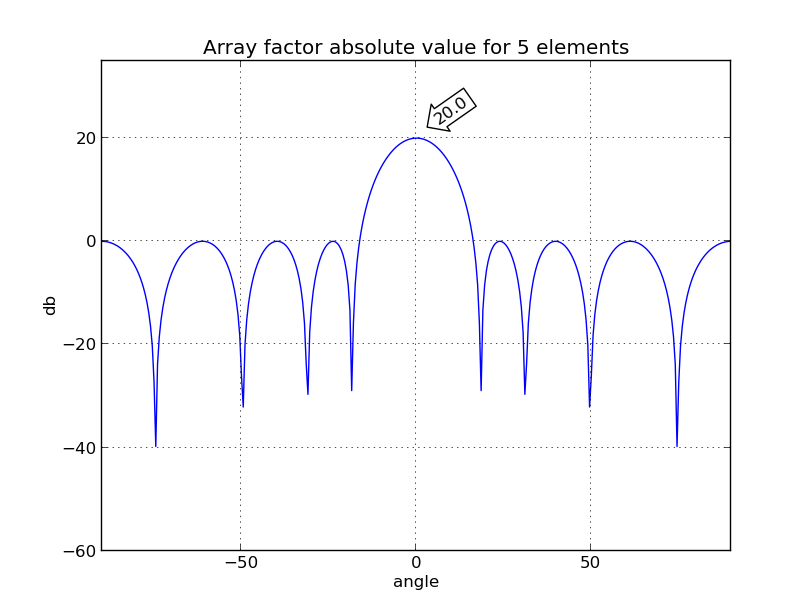
\includegraphics[scale=0.5]{Immagini/module5}
\end{figure}
\begin{figure}
\centering
\caption{Modulo del fattore di array per M = 7.}
\label{img:module7}
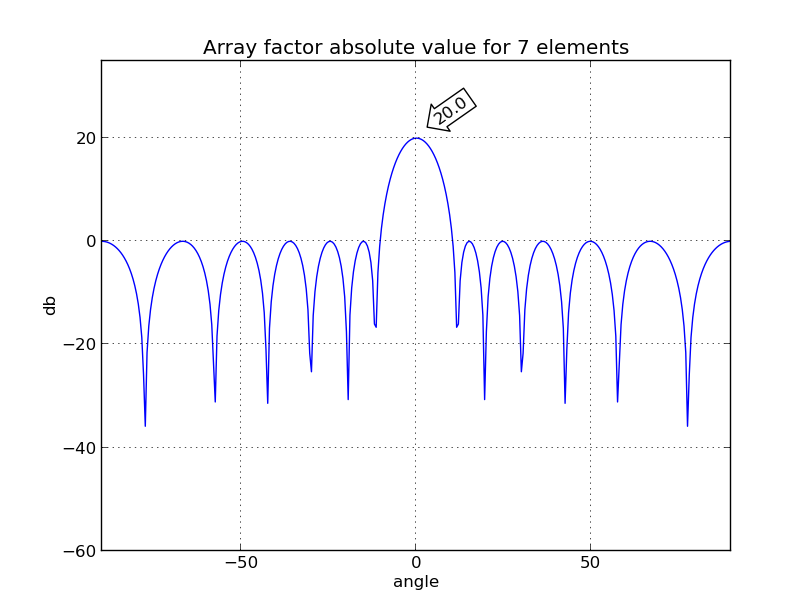
\includegraphics[scale=0.5]{Immagini/module7}
\end{figure}
\begin{figure}
\centering
\caption{Modulo del fattore di array per M = 9.}
\label{img:module9}
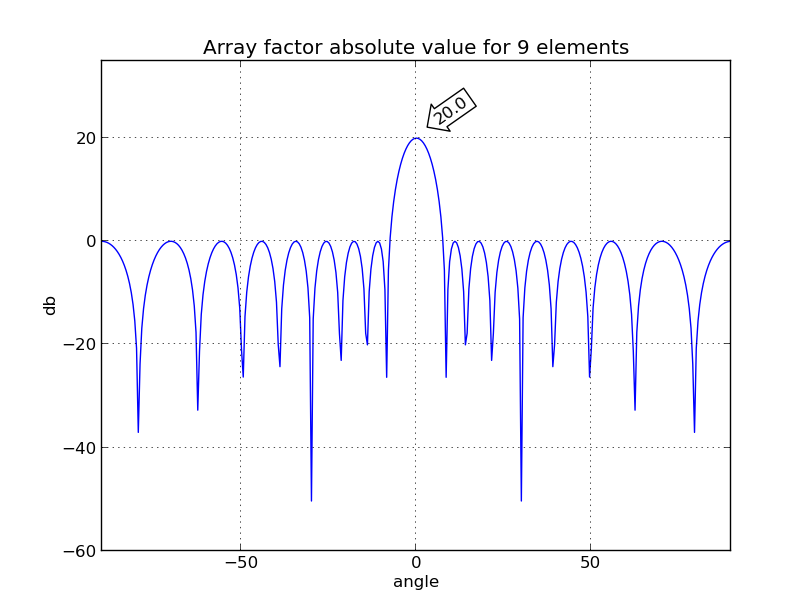
\includegraphics[scale=0.5]{Immagini/module9}
\end{figure}

Per quanto riguarda il guadagno totale del patch e dell'array (Fig. \ref{img:gain5}, \ref{img:gain7}, \ref{img:gain9}), si può vedere come all'aumentare di $M$ diminuisca la larghezza dei lobi (in particolare di quello principale) e aumenti il numero di lobi secondari. Molto importante è anche l'aumento del guadagno che arriva ad un valore prossimo a $16 dB$ (come previsto dalle specifiche) per $M = 9$, avendolo impostato nella relazione (\ref{eq:m}). \\ 

\begin{figure}
\centering
\caption{Guadagno totale per M = 5.}
\label{img:gain5}
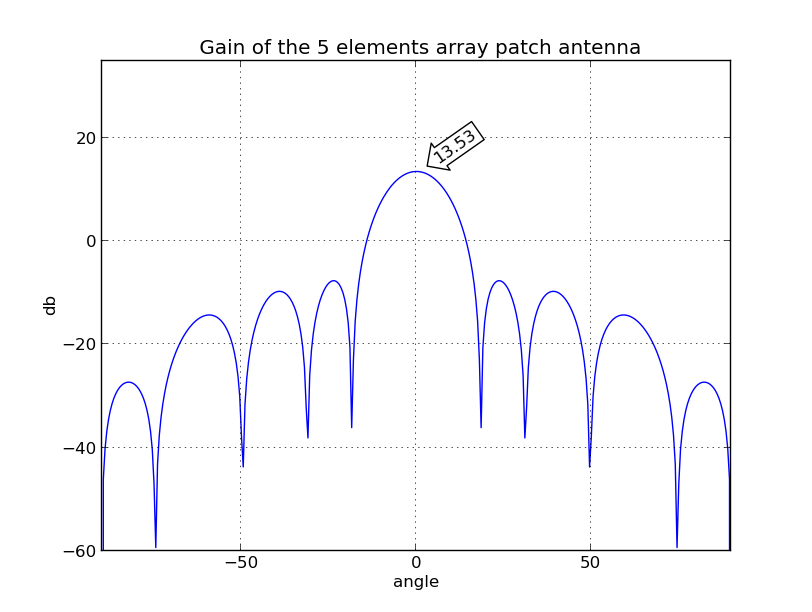
\includegraphics[scale=0.5]{Immagini/gain5}
\end{figure}
\begin{figure}
\centering
\caption{Guadagno totale per M = 7.}
\label{img:gain7}
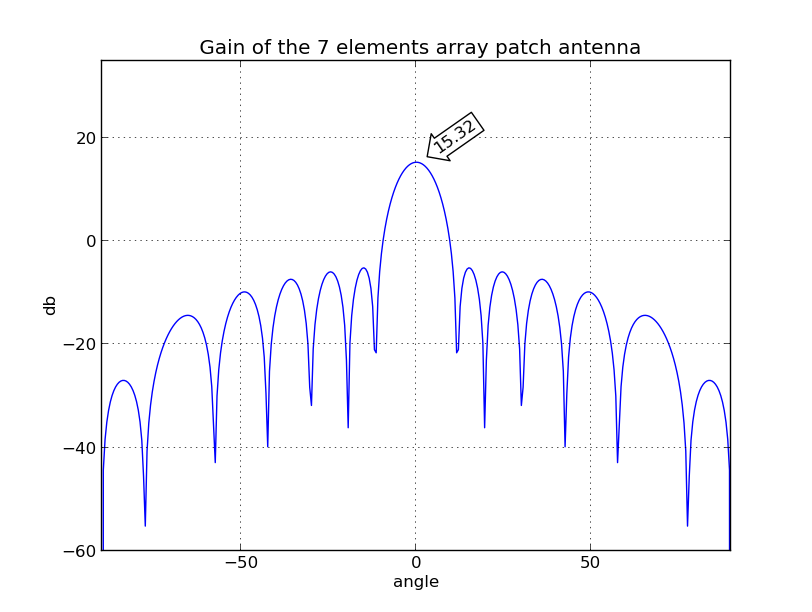
\includegraphics[scale=0.5]{Immagini/gain7}
\end{figure}
\begin{figure}
\centering
\caption{Guadagno totale per M = 9.}
\label{img:gain9}
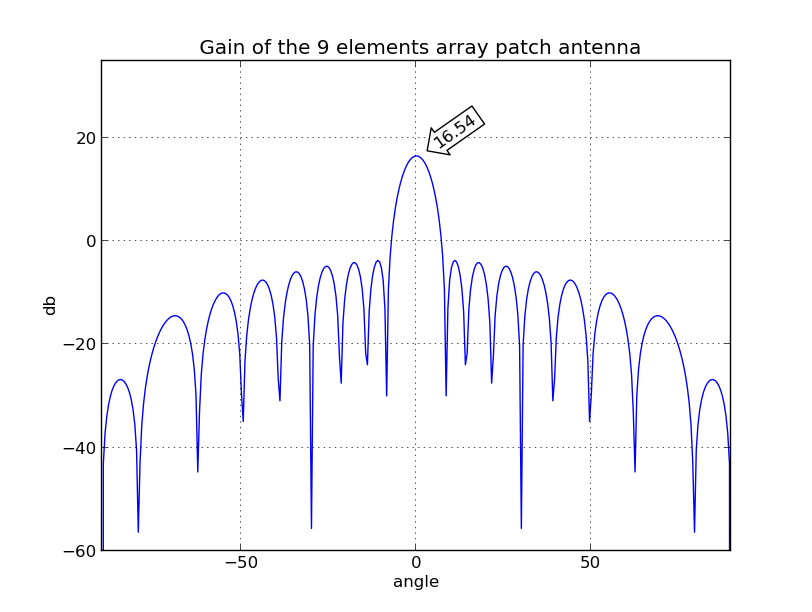
\includegraphics[scale=0.5]{Immagini/gain9}
\end{figure}


Infine è stata fatta variare la distanza tra gli elementi dell'array (tra $\frac{\lambda}{2}$ e $\lambda$) ed è stato rappresentato il beamwidth; in ognuno dei tre grafici è stata considerata una diversa cardinalità degli elementi degli array, $M = 5$ (Fig. \ref{img:bw5}), $7$ (Fig. \ref{img:bw7}), $9$ (Fig. \ref{img:bw9}). \\
Si può notare chiaramente come il \emph{beamwidth} diminuisca all'aumentare della distanza tra gli elementi. Per capire se sia soddisfatta la specifica sull'angolo a metà potenza è necessario controllare il valore di $10^\circ$ del \emph{beamwidth}: nel caso di $M = 5$ nel range considerato di $d$ non è possibile trovare il \emph{beamwidth} richiesto, al contrario che nelle altre due configurazioni. In particolare si può notare come nel caso di $M = 9$ la scelta di $d$ sia diversa da quella calcolata con la (\ref{eq:d}) ma nonostante questo, si può scegliere il relativo valore a $B = 10^\circ$, in quanto le specifiche su $R$ e su $G$, restano soddisfatte perché indipendenti dalla distanza $d$. \\[1cm]
\begin{figure}
\centering
\caption{Angolo a metà potenza per M = 5.}
\label{img:bw5}
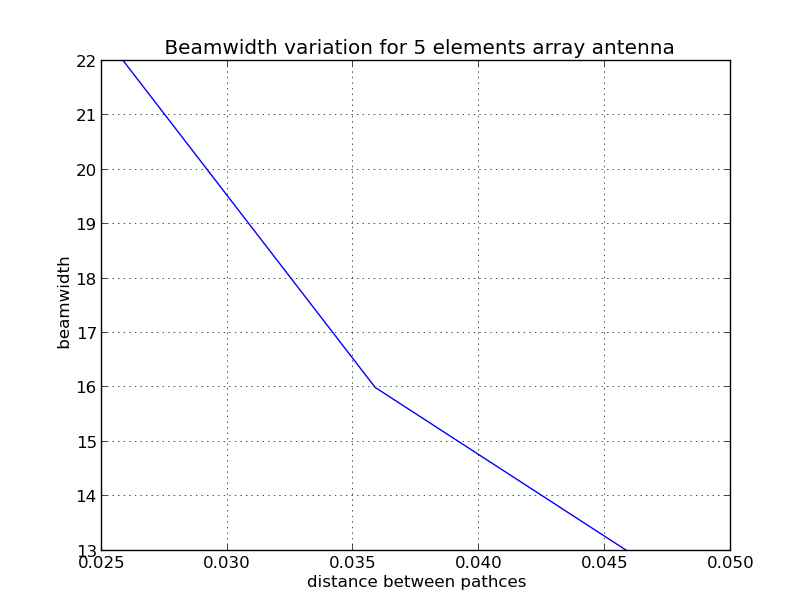
\includegraphics[scale=0.5]{Immagini/bw5}
\end{figure}
\begin{figure}
\centering
\caption{Angolo a metà potenza per M = 7.}
\label{img:bw7}
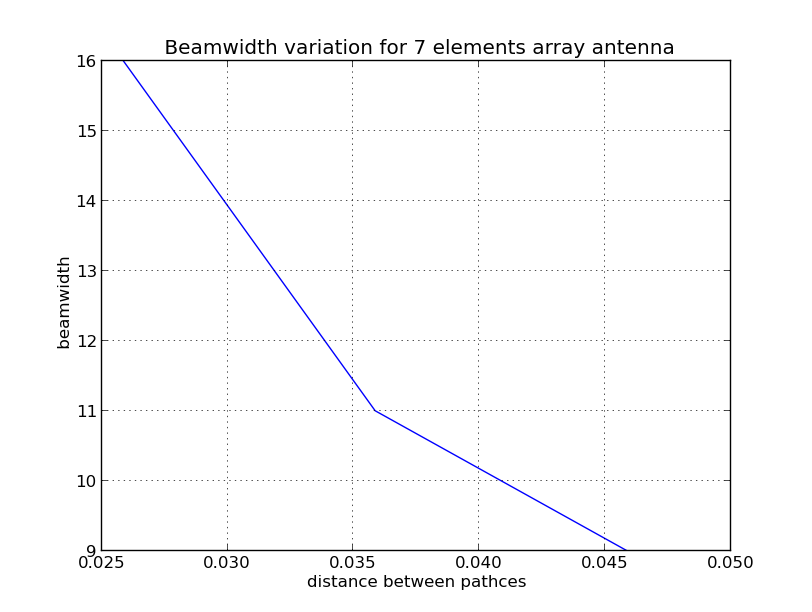
\includegraphics[scale=0.5]{Immagini/bw7}
\end{figure}
\begin{figure}
\centering
\caption{Angolo a metà potenza per M = 9.}
\label{img:bw9}
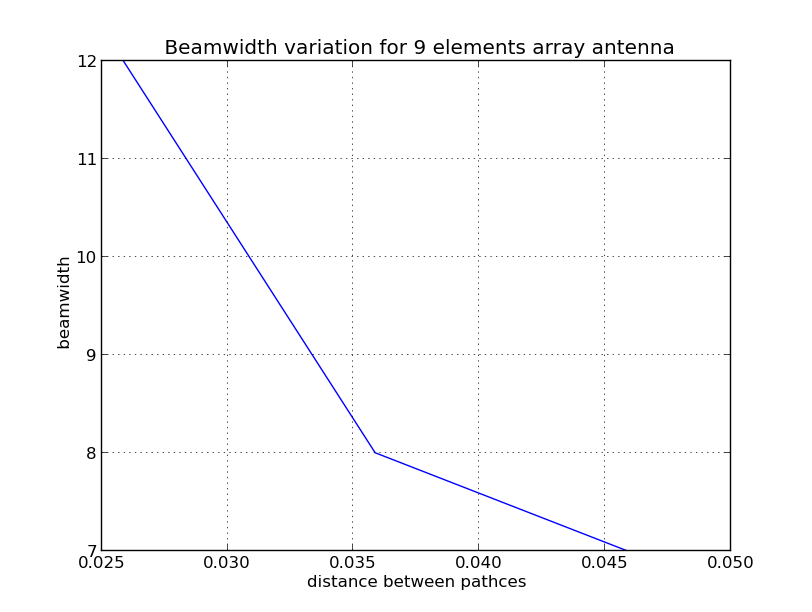
\includegraphics[scale=0.5]{Immagini/bw9}
\end{figure}

Nella tabella \ref{tab:dgbopt} sono riassunti i risultati ottenuti nelle tre tipologie di grafico rappresentate nelle pagine precedenti, in funzione della cardinalità degli elementi dell'array.
\begin{table}[h]\footnotesize
\caption{Risultati al variare di M.}
\label{tab:dgbopt}
\begin{tabularx}{\textwidth}{XXXX}
\toprule
& $M = 5$ & $M = 7$ & $M = 9$ \\
\midrule
Distanza ottima (m) & 0.0404149389796 & 0.043831493932 & 0.0457028645254 \\
Guadagno max	 (dB) & 13.53 & 15.32 & 16.54 \\
Beamwidth & $14.0^\circ$ & $9.0^\circ$ & $7.0^\circ$ \\
\bottomrule
\end{tabularx}
\end{table}
